\documentclass[
    coverheight=148mm, coverwidth=105mm, spinewidth=10mm,
    bleedwidth=31mm,
    foldingmargin=true, 12pt
]{bookcover}

\usepackage{ebgaramond-maths}
\usepackage{microtype}

\begin{document}
\begin{bookcover}
    \bookcovercomponent{normal}{front}{
        \centering
        \vfill
        {\Huge The Archer's Revenge}
        \vfill
        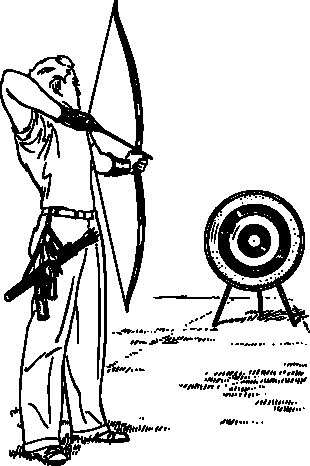
\includegraphics[width=0.5\partwidth]{frontcover-bw-image.pdf}
        \vfill
        {\Large Destination Infinity}
        \vfill
    }
    \bookcovercomponent{normal}{back}[5mm,,5mm,]{
        \setlength{\parskip}{1ex}
        \vfill
        Destination Infinity is the online identity of Rajesh Kollu, who is basically a
        'Professional' Blogger living in Chennai, India. He has an opinion on everything
        and is an expert on nothing!

        He was forced to become an author because people kept pestering him with the
        lethal question, 'What do you do?'.

        When he answered, 'I am a professional blogger', people usually replied with
        questions like, 'What is a professional blogger? I have never heard of this? Do
        you know anyone who is *also* a professional blogger? Will anyone in their
        senses become a professional blogger? You quit your *plum* sales career for
        this? Do you earn anything out of your work? How do you eat?', etc.

        Now, since (at least) one of his books has been (self) published, both as an
        ebook and on paper, he can safely
        say, 'I am an author, I write book(s)'. With that one sentence, he aims to
        eliminate any further questions, especially the 'Do you earn anything out of
        your work?'.

        Because, it's quite normal to be an author and not be earning anything at all!!
        :D

        You can follow his misadventures at

        \centerline{http://www.destinationinfinity.org}

        \vfill

        \begin{center}
            
\includegraphics[width=18pt]{logo.pdf}
        \end{center}
    }
\end{bookcover}
\end{document}